\documentclass[12pt,titlepage,a4paper]{report}
% Texte
\usepackage[utf8]{inputenc}
\usepackage[T1]{fontenc}
\usepackage[french]{babel}
\usepackage{lmodern}
\usepackage{float}
\usepackage{enumitem}
\usepackage{minted}
\usemintedstyle{trac}

% Pour les checkmarks
\usepackage{pifont}
\usepackage{amssymb}
% Pour des \hline en gras
\usepackage{makecell}
% Numéroter les chapitres à partir de chaque début de partie
\makeatletter\@addtoreset{chapter}{part}\makeatother

% Mise en page
\usepackage{url}
\usepackage[top=2.1cm,bottom=2cm,left=3cm,right=3cm]{geometry}
\usepackage{hyperref}
\hypersetup{
    colorlinks=false,
    pdfborder={0 0 0},
}
\usepackage{multirow}

% TOC
\usepackage[french]{minitoc}
\setcounter{tocdepth}{2}
\setcounter{minitocdepth}{2}
\setlength{\mtcindent}{0pt}

% Images
\usepackage{float}
\usepackage{wrapfig}
\usepackage{graphicx}
% Pour inclure des pages PDF
\usepackage[final]{pdfpages}

% Couverture
\usepackage{templateINSA}
\initINSA

% Citations
\usepackage{epigraph}
\setlength\epigraphwidth{12cm}
\setlength\epigraphrule{0pt}

\usepackage{etoolbox}

\makeatletter
\patchcmd{\epigraph}{\@epitext{#1}}{\itshape\@epitext{#1}}{}{}
\makeatother

\usepackage[nottoc, notlof, notlot]{tocbibind}

\title{Reconnaissance de caractères et détection de langue}
\author{Manon \bsc{Ansart}\\ Anthony \bsc{Courtin}}

\renewcommand\soustitre{Rapport de projet}
\renewcommand\infoBig{Projet d'Approfondissement et d'Ouverture}
\renewcommand\infoSmall{ASI4 2014-2015}
\newcommand{\code}[1]{\texttt{#1}}
\newcommand{\hlineGras}{\Xhline{2\arrayrulewidth}}

\def\changemargin#1#2{\list{}{\rightmargin#2\leftmargin#1}\item[]}
\let\endchangemargin=\endlist 

\begin{document}
	\titleINSA{15}{images/fond.jpeg}{0}{0}{300}{\href{http://img0.gtsstatic.com/wallpapers/92e875b279aa0e52dc1b5cc12443416a_large.jpeg}{\textcolor{white}{CC - Istockphotos}}}

	\dominitoc
	\tableofcontents

	\chapter{Introduction}
		Le but initial de ce projet était de travailler avec la librairie Olena d'Epita afin de détecter des photos dans des images de documents. Après le téléchargement et la compilation de la librairie, nous avons tenté de la tester et de rechercher les fonctions utiles pour l'application que nous voulions en faire. Nous avons découvert que la librairie était bien plus complexe que ce que nous pensions, et qu'elle ne fournissait pas de fonction permettant de trouver directement une photo dans une image. Nous avons donc décidé de choisir un autre sujet, toujours dans le cadre de la reconnaissance d'image de document. Pendant ce Projet d'Approfondissement et d'Ouverture, nous allons utiliser la bibliothèque ocropus pour reconnaître les caractères à partir d'une image de documents puis en détecter la langue grâce au module de détection de langue cld2 développé par google.

	\chapter{Compréhension des outils}
		\section{Ocropus}
			\subsection{Généralités}
	OCRopus est un logiciel libre de reconnaissance optique de caractères (ROC) ou optical character recognition (OCR) en anglais. Il a pour but de pouvoir être utilisé à la fois par des chercheurs et des entreprises\cite{articleOCRopus}, c'est pourquoi il a été développé sous licence Apache 2, qui permet une utilisation commerciale facile. 

	OCRopus permet d'utiliser plusieurs modules de reconnaissance de texte. En particulier, il implémente Tesseract, qui est considéré comme un des modules les plus exactes dans le domaine des logiciels libres. Ces performances se rapprochent de celles des modules commerciaux peu connus.

\subsection{Fonctionnement}
	OCRopus, comme n'importe quel logiciel d'OCR, fonctionne selon 5 étapes principales \cite{articleOCRopus} : Le pré-traitement, l'analyse de page, la reconnaissance des caractères, le post-traitement puis la mise en forme du résultat

	\subsubsection{Pré-traitement}
		Cette étape a pour but de traiter l'image d'entrée afin de faciliter les étapes suivantes. Cela implique par exemple de redresser une image inclinée, de travailler sur le contraste... OCRopus fourni une toolbox pour les images en noir et blanc ou niveau de gris.

	\subsubsection{Analyse de page}
		Une fois l'image optimisée pour le traitement, elle est découpée en lignes de texte. Pour cela, OCRopus recherche d'abord la présence de colonnes, puis découpe chacune de ces colonnes en lignes. Ces lignes pourront ensuite être traitées séparément

	\subsubsection{Reconnaissance de caractère}
		Les lignes en sortie de l'étape précédente sont analysées afin d'en reconnaître les différents caractères. Pour se faire, les images de caractères sont analysées une à une et comparées par différentes méthodes a des images de caractères connus dans une base de donné. Le ou les caractères les plus proches sont choisis. C'est dans cette partie que Tesseract est utilisé.

	\subsubsection{Post-traitement}
		Une analyse statistique est ensuite utilisée pour améliorer le résultat et lever les éventuelles ambiguïtés. Des dictionnaires sont utilisés pour calculer la probabilité de séquences de lettres, ce qui permet de poser un modèle linguistique utilisé dans cette étape.

	\subsubsection{Mise en forme}
		Les lignes ayant été analysées une par une, une dernière étape est nécessaire afin de mettre en forme les différents résultats obtenus afin d'obtenir une résultat final unique : une page html contenant le texte de sortie. Un script bash nous permet de convertir cet page html en un fichier txt. 


\subsection{Résultats}
	
	Nous avons tenté d'utiliser OCRopus pour obtenir le texte présent dans différentes images. 

	\begin{figure}[H]
		\centering
		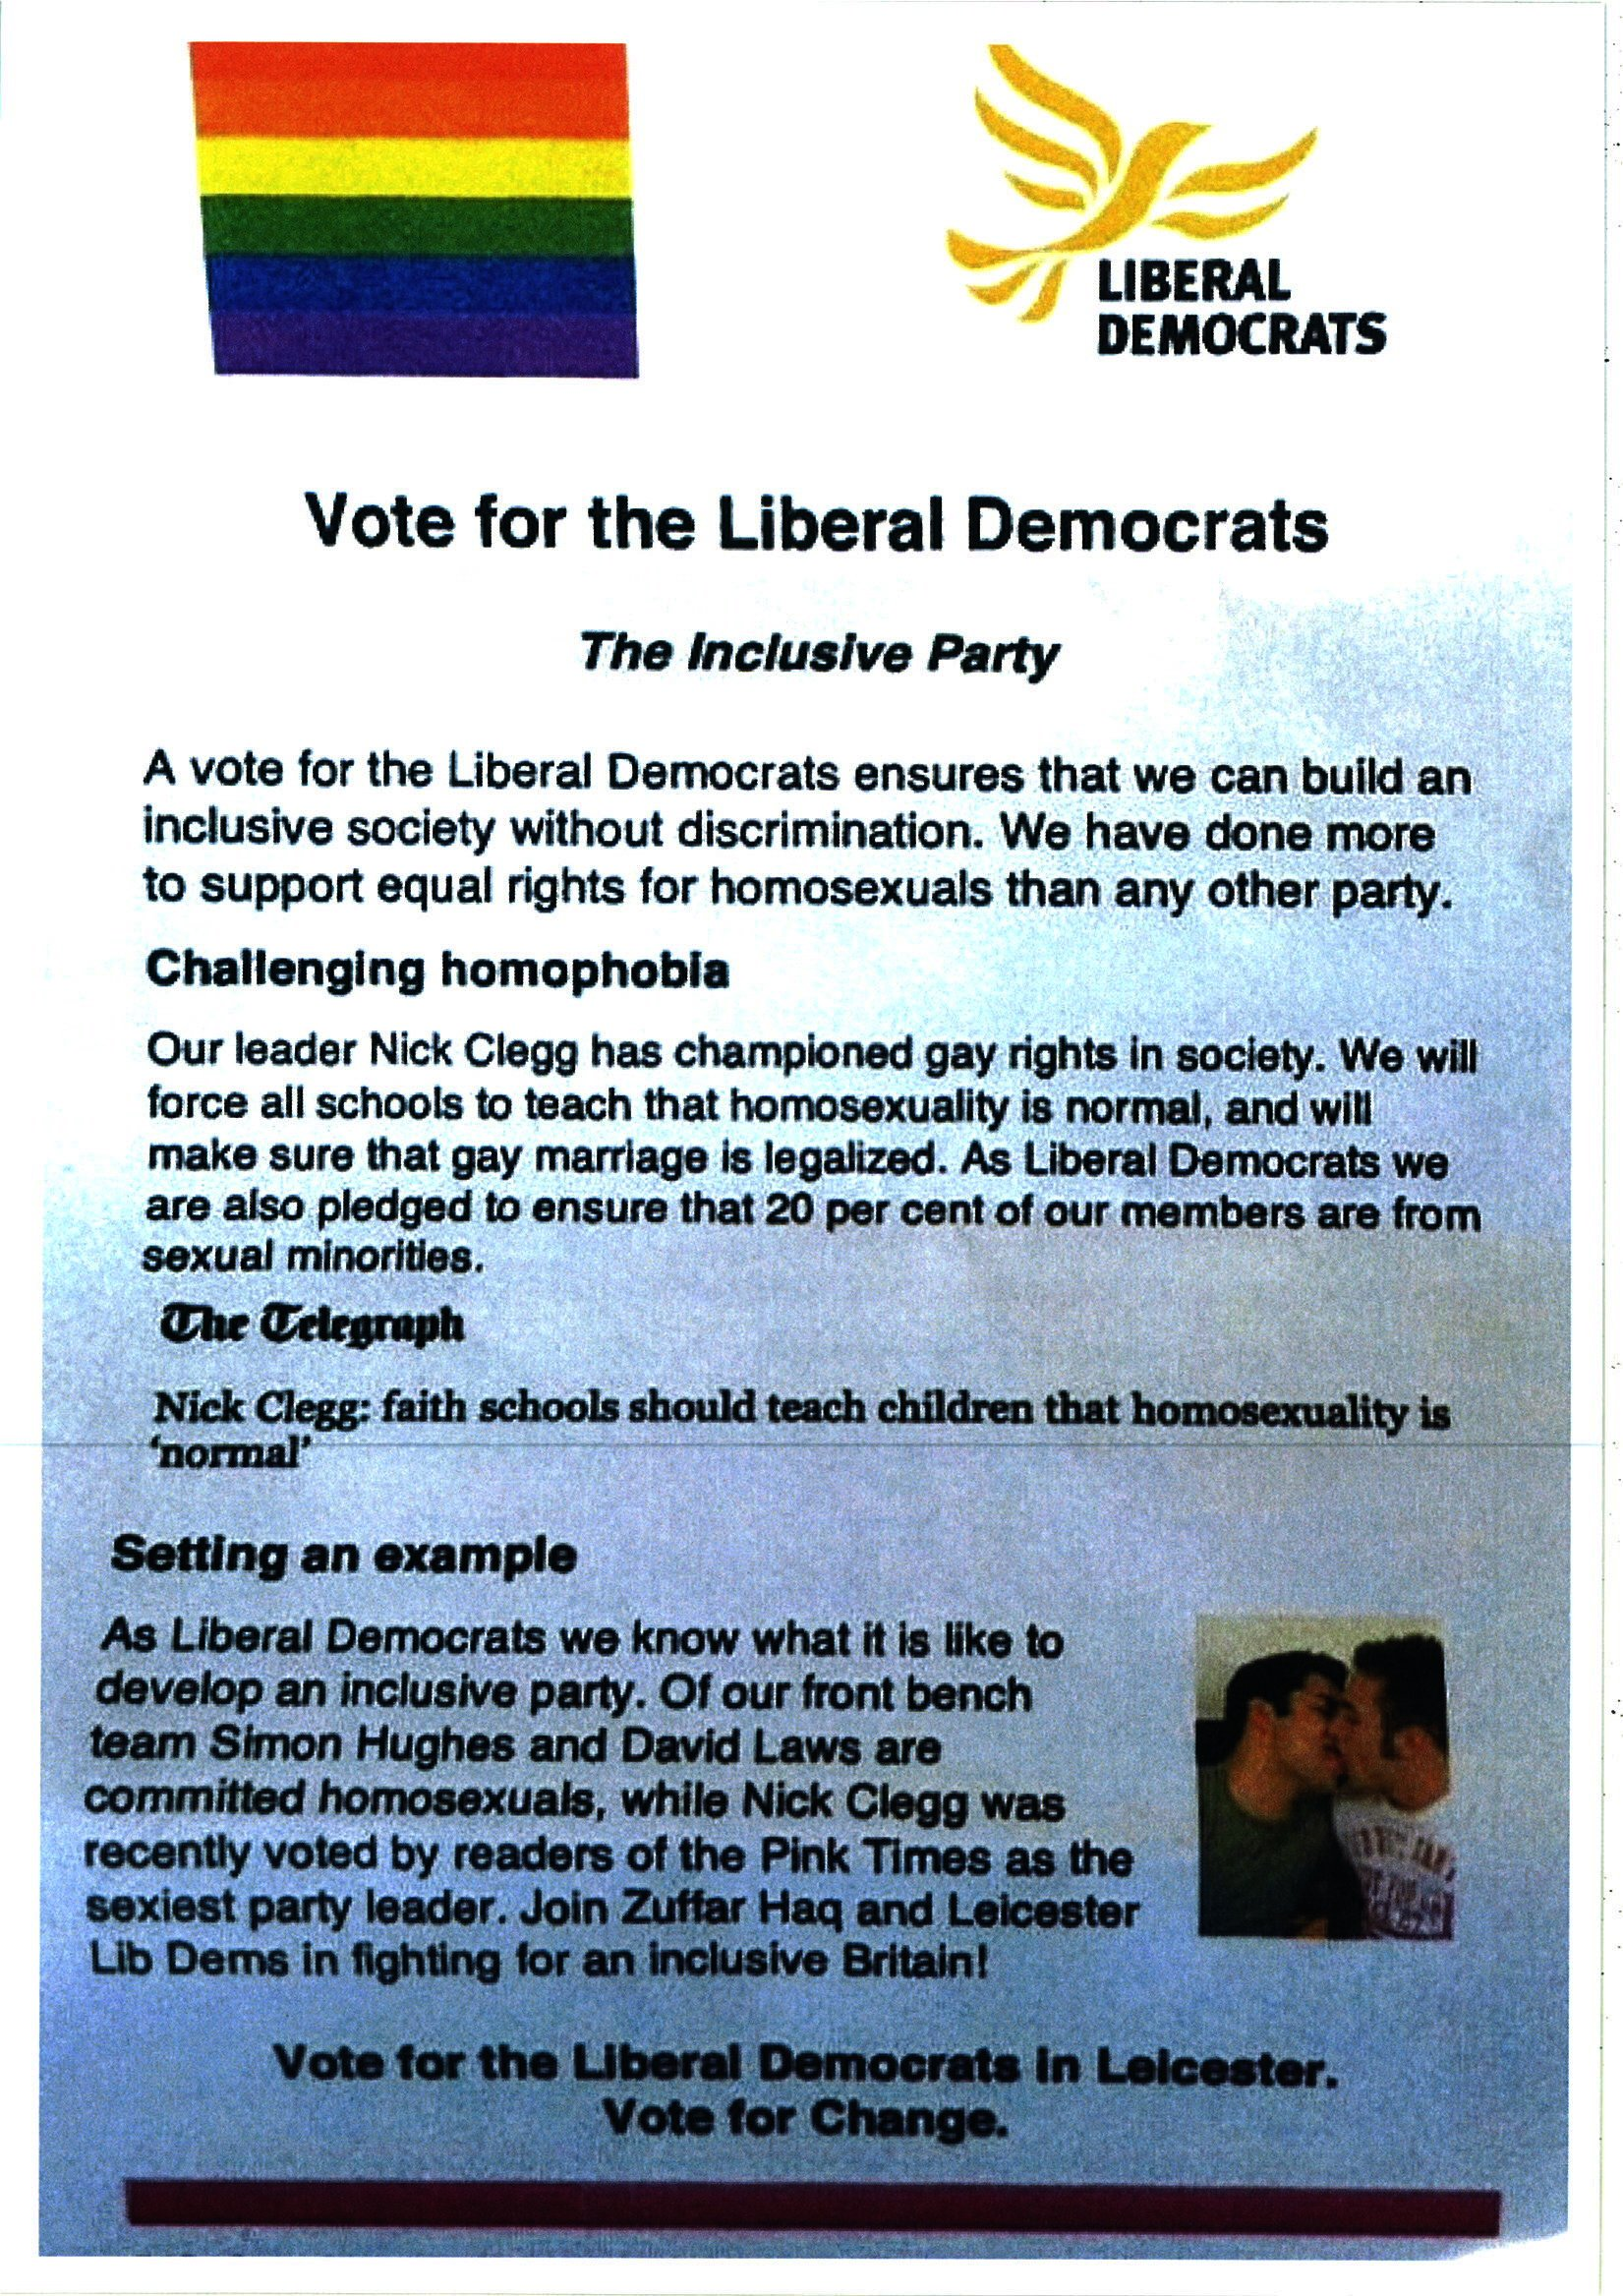
\includegraphics[scale=0.4]{images/FJEZNU.jpg}
		\caption{Image à traiter par OCRopus}
		\label{fig:image}
	\end{figure}

	\begin{figure}[H]
		\centering
		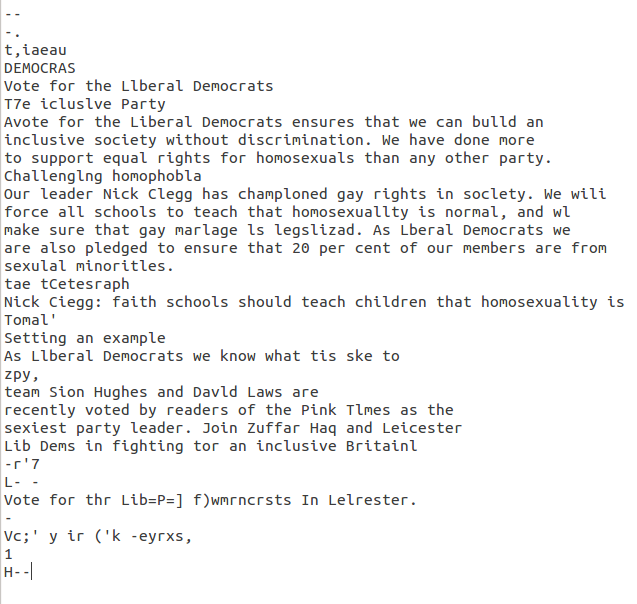
\includegraphics[scale=0.6]{images/FJEZNU_result.png}
		\caption{Texte trouvé par OCRopus}
		\label{fig:resultat}
	\end{figure}

	Avec cette image, on remarque que les lettre se ressemblant (i et l) sont souvent confondues, et que la qualité de l'image est importante : le bas de la page, moins bien éclairé, est mal reconnu et le mot "normal", situé sur la pliure, est interprété comme Tomal'. On remarque également que la police est importante : The Telegraph est interprété comme tae tCetesraph.

	Des essais sur d'autres images nous ont montré que la rotation est importante (une image tournée à 90 $\deg$ n'est pas du tout reconnue par OCRopus) ainsi que l'espacement entre les caractères, qui peut rendre la police plus ou moins "lisible". Enfin, les écritures manuscrites ne sont pas du tout reconnues pas OCRopus.



		\section{Cld2}
			\subsection{Généralités}
	CLD2, ou Compact Language Detection 2, est un package proposé par google \cite{googleCodeCLD2} pour detecter la langue d'un texte, fourni sous la forme d'une chaine ou d'une page HTML/XML. Comme son nom l'indique, il fait suite à CLD en y ajoutant plusieurs améliorations et des nouveautés, comme des langues supplémentaires (CLD2 peut en detecter 83 différentes, nous ne les listerons pas toutes ici) et la possibilité d'obtenir en sorti le texte correspondant aux 3 langues principales quand plusiquers langues sont detectées, pour pouvoir par exemple tout traduire dans une même langue.

	CLD2 a été créé pour travailler sur des pages web comprenant plus de 200 caractères. De ce fait, des "indices", tels que des balises html concernant la langue ou le Top Level Domain de l'URL (.fr, .de ...) sont utilisés pour influcencer les résultats du package. Étant donné que nous n'utiliserons pas CLD2 sur des pages web mais sur des chaines de textes extraites par Ocropus, ces indices ne seront pas utilisés dans notre cas.

\subsection{Nettoyage des données}
	La première étape effectuée par CLD2 afin de travailler sur le texte et détecter la langue est de nettoyer le texte fourni pour pouvoir le traiter. 

	Tout d'abord, tout le texte est passé en minuscule. Ensuite, tous les nombres, la ponctuation et les tags html, non utiles pour la détections de la langue, sont supprimés. Les mots d'une seule lettre sont également ignorés. 

	Les mots sont séparés en séquences de 4 lettres, appelés quadrigramme. Le signe \_ est ajouté au début ou à la fin du quadrigramme pour indiquer que ce quadrigramme se trouve au début ou à la fin du mot, ce qui peut être caractéristique d'une langue.

	Les mots qui ne sont pas caractéristiques d'une langue et pouvant biaiser la detection, tels que les extensions (.jpg, .gif, ...) sont supprimés.

\subsection{Analyse statistique}
	Une fois les données nettoyées, une analyse statistique peut être effectuée sur le texte afin d'en détecter la langue. On travaillera sur les quadrigramme créé précédemment.

	La méthoe utilisée est probabiliste. Une table contenant des entrées de 4 bytes est utilisée afin d'associer à chaque quadrigramme entre 3 et 6 langues les plus probables. Un "score" est alors calculé à partir de la probabilité logarythmique du quadrigramme pour ces langues.

	La table contenant les langues et les probabilités a été créée à partir d'un corpus de texte. Dans un premier temps, des pages web en chacune des langues ont été choisies humainement et traitées. 100 milions de pages web choisies automatiquement ont ensuite été ajoutées. 


\subsection{Résultats}

	\begin{itemize}
		\item "Bonjour, vive notre PAO" : FRENCH(95\% 1291p)
		\item "Nous sommes ravis de vous rencontrer." : FRENCH(97\% 885p)
		\item "Hello, nice to mee you too" :  ENGLISH(96\% 1175p)
		\item "Nous sommes ravis de vous rencontrer. Hello, nice to meet you too. " : Unknown(un-reliable). On constate que 2 phrases dans deux langues différentes qui sont bien detectées séparemment ne sont pas bien detectées lorsqu'elles sont ensemble.
		\item "Nous sommes ravis de vous rencontrer. Visiblement il faut beaucoup plus de texte pour pouvoir detecter la langue. Hello, nice to meet you too." : FRENCH(99\% 633p)
		\item "Nous sommes ravis de vous rencontrer. Visiblement il faut beaucoup plus de texte pour pouvoir detecter la langue. Hello, nice to meet you too. We need to put a little more text here too. Let's hope it works." : FRENCH(56\% 772p), ENGLISH(43\% 1314p). Il nous fout plus de texte dans chaque langue quand 2 langues sont mélangées.
		\item "Il se rague roupète drâle emparouille endosque pratèle libucque barouffle ouillais tocarde marmine manage" : Unknown(un-reliable). En mettant des mots n'existant pas mais à sonorité française (extraits du poème Le Grand Combat d'Henri Michaux), on s'attendrait à ce que CLD2 trouve la langue français mais ce n'est pas le cas. CLD2 n'est pas si facile à berner !
		\item "Essayons de trouver" : FRENCH(95\% 870p). 3 mots français peuvent suffire pour detecter la langue, ce qui est mieux que les 200 mots minimum prévus.
		\item "esrdtu Essayons eghedu de eedef trouver kjhgvb jjkkl zzza" : FRENCH(98\% 300p). L'ajout de séquences de lettres aléatoires ne perturbent pas beaucoup CLD2
		\item "Essayons de troujver" : Unknown(un-reliable). Le fait de modifier un mot perturbe en revanche beaucoup le résultat.
	\end{itemize}

	

	\chapter{Conception de l'application}
		\section{L'application Android}
			\subsection{Conception}

Nous avons développé cette application pour les systèmes d'exploitation Android. La programmation pour Android est basée sur le langage java que nous avons vu l'année dernière en cours de programmation avancée. Néanmoins, même si nous possédions de bonnes bases java, il nous a fallu plusieurs semaines afin de savoir développer sur Android car celui-ci fonctionne différemment du langage java que nous avions pu voir. \\

Une fois le langage assimilé, nous nous sommes attaqué à la conception de l'application. Nous avons tout d'abord élaboré un dessin papier des différentes vus de notre application. Au fur et à mesure que nous avancions dans le developpement nous nous sommes rendu compte qu'il serait plus compliqué que prévu de réaliser toutes ces vus. Nous avons donc opté pour une application plus simple mais qui réppond à nos attentes.\\

la figure ci dessous présente le menu de démarrage de l'application : 
	\begin{figure}[H]
		\centering
		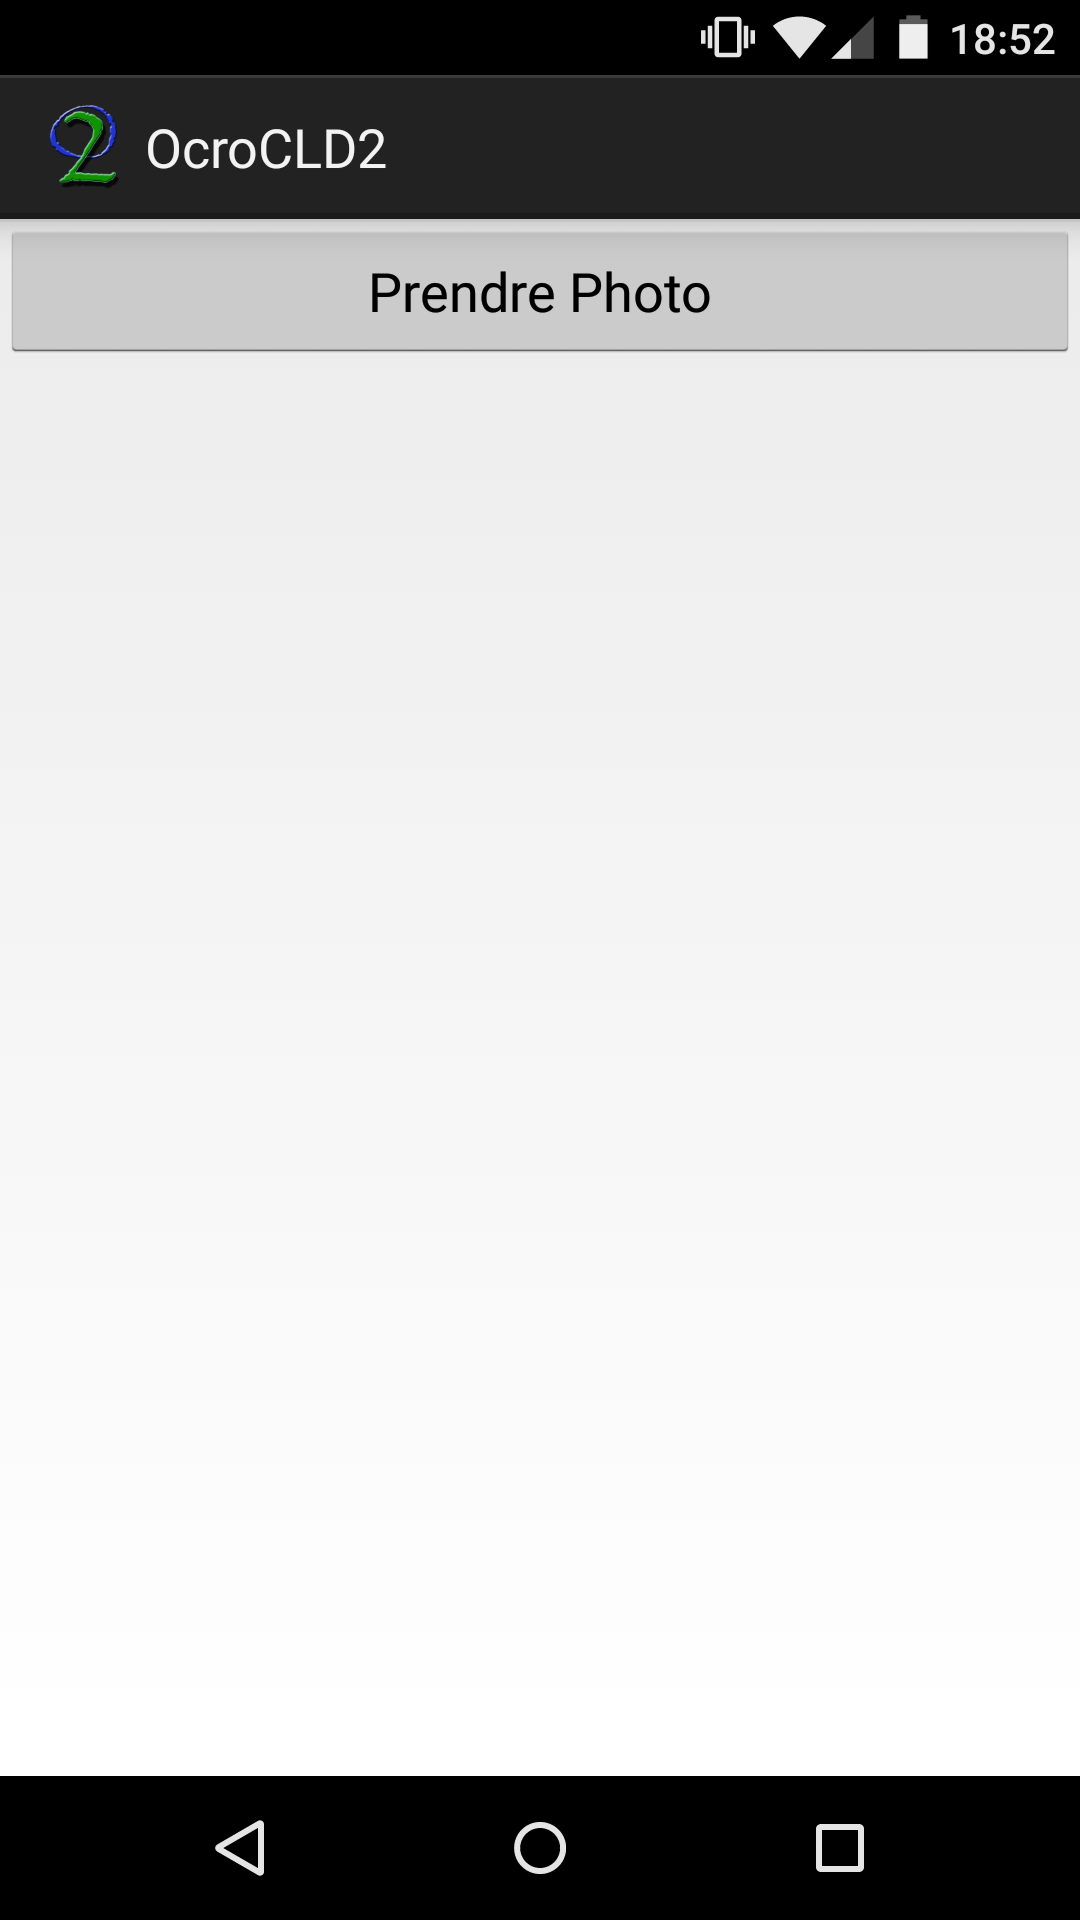
\includegraphics[scale=0.1]{images/appliMenu.png}
		\caption{Menu principal}
		\label{fig:image}
	\end{figure}

\subsection{Fonctionnement}
L'intégralité du code de l'application est disponible dans l'archive fournis.\\

Lorsque nous sommes dans le menu principal il nous suffit d'appuyer sur le bouton "prendre une photo" afin que l'application fasse appelle à l'application appareil photo de notre mobile. Pour faire ceci, nous utilisons un listener qui lorsque l'on clic sur le bouton l'applcation crée un intent afin d'utiliser l'application en charge des photos. Ceci nous à permis de ne pas redévelopper l'appareil photo déjà présent.\\

Une fois que nous avons pris la photo, il nous suffit de valider et nous retournons à l'accueil. L'application envoie alors grâce à notre classe DataSender l'image par protocole Http sur l'adresse du script php de notre serveur. Une fois cela fait, l'application reste à l'écoute du serveur afin de récupérer la chaine de caractère renvoyée. Cette chaine contient le résultat du traitement par Ocropus puis CLD2.\\

Nous pouvons alors reprendre une photo ou bien quitter l'application.

\subsection{Problèmes rencontrés}

Tout d'abord, l'apprentissage du java pour Android est apparu plus difficile que prévu car nous ne pensions pas qu'il y avait autant de différences. De plus nous avons eu quelques soucis pour installer le SDK android sur Eclipse. C'est pourquoi nous avons pris un peu de retard au début de ce projet.\\

Ensuite, il a été assez compliqué de faire communiquer l'application avec le serveur. Plus précisément, nous ne savions pas quel type de protocole était le plus adapté afin d'envoyer une photo sur un serveur. Après avoir consulté Mr Nicolas Malandin, nous avons donc opté pour le protocole Http.\\

Finalement, nous avons toujours des problèmes de réponse du serveur, ce qui fait que par moment nous ne sommes pas certain de recevoir une réponse. En effet, le traitement de l'image par Ocropus prend plusieurs minutes suivant la taille du texte à traiter.

		\section{La communication avec le serveur}
			\subsection{Connection au serveur}

Afin d'installer et de faire nos tests nous nous connectons en ssh sur un serveur que Mr Sebastion Bonnegent nous a mis à disposition : \textit{ssh -X paoandroid@asi-android.insa-rouen.fr}.
De plus, il faut se trouver sur le réseau WEP-26 de l'INSA de Rouen pour pouvoir se connecter. Lorsque le PAO sera terminé, le serveur sera fermé, il faudra donc redemander un serveur pour pouvoir reprendre le projet.

\subsection{Installation des outils}

\subsubsection{Ocropus}

\begin{itemize}
 \item Dans un premier temps, il faut cloner le répertoire d'Ocropus à l'aide de la commande : \textit{hg clone -r ocropus-0.7 https://code.google.com/p/ocropus};
 \item Si cela ne fonctionne pas, il faut installer le package que linux vous suggère;
 \item Ensuite, déplacez vous dans le dossier ocropy : \textit{cd ocropus/ocropy};
 \item Installez les packages nécessaires au fonctionnement : \textit{sudo apt-get install \$(cat PACKAGES)};
 \item Téléchargez les modèles python : \textit{python setup.py download\_models};
 \item Lancez l'installation : \textit{sudo python setup.py install};
 \item Lancez les tests : \textit{./run-test};
 \item Si tout est correctement installé, vous devriez avoir un message d'Ocropus disant que vous pouvez visualiser les résultats en tapant une certaine ligne de commande.
\end{itemize}

\subsubsection{CLD2}

\begin{itemize}
 \item Allez dans votre dossier tmp : \textit{cd /tmp/};
 \item Téléchargez le répertoire de CLD2 : \textit{svn checkout http://cld2.googlecode.com/svn/trunk/cld2};
 \item Déplacez vous dans le dossier internal : \textit{cd cld2/internal};
 \item Copiez et collez le fichier compile\_libs\_32bit.sh dans le répertoire internal (ce fichier est joint dans l'archive que nous avons fourni). Celui-ci sert à pouvoir exécuter CLD2 dans un terminal;
 \item Autorisez l'exécution de ce fichier : \textit{chmod u+x compile\_libs\_32bit.sh};
 \item Exécutez le fichier : \textit{./compile\_libs\_32bit.sh};
 \item Effectuez le test suivant dans votre terminal : \textit{echo "Hello World je suis gentil trop bien my name is i don't know" | cld2};
 \item Si tout est correctement installé votre terminal affichera un message vous disant que le texte est en anglais et français.
\end{itemize}

\subsubsection{Lynx}

Il faut installer lynx qui permet de convertir une page html en fichier txt : \textit{sudo apt-get install lynx}.

\subsection{PHP}
Comme dit précédemment, l'application envoie l'image au serveur par protocole Http directement sur un script php qui, lorsqu'il reçoit l'image, la copie dans le bon dossier et lance les différentes commandes nécessaires au traitement de l'image. Ce script est disponible dans l'archive fournie. Une fois que Ocropus a fini CLD2 est exécuté et renvoie une chaîne de caractère transmise à l'application par protocole Http.

\subsection{Problèmes rencontrés}

Le premier problème que nous avons rencontré avec le serveur vient d'Ocropus. En effet, lorsque celui-ci est exécuté, il ouvre une fenêtre graphique afin de traiter les images. Celle-ci n'est pas visible à l'écran mais empêche le bon fonctionnement d'Ocropus, d'où le -X dans la commande permettant de se connecter au serveur qui permet de se servir de notre écran comme écran miroir.\\
Afin de résoudre ce problème nous avons modifié quelques lignes de code des bibliothèques d'Ocropus afin que celui-ci n'ouvre plus de fenêtre graphique pour exécuter le script bash directement grâce à une requête HTML et ne plus avoir de message d'erreur. Afin de savoir quel fichier modifer, il faut se connecter au serveur sans le -X et exécuter Ocropus.\\
Voici les trois lignes de code à rajouter au tout début du fichier :
\begin{itemize}
 \item import matplotlib
 \item matplotlib.use('Agg')
 \item import matplotlib.pyplot
\end{itemize}
Si le problème persiste après c'est que vous n'avez pas modifié le bon fichier python.\\

Le deuxième problème fut les droits d'accès aux fichiers. En effet, lorsque l'application android envoie la requête sur le script php du serveur, ce script est exécuté par Apache. Il faut donc que Apache possède les droits d'accès, de modification et d'exécution sur les dossiers d'Ocropus et tous ceux nécessaires au bon fonctionnement du script.\\
Pour résoudre ce problème nous avons donnés les droits root à Apache ce qui ne constitue pas forcément la meilleure des solutions car très risquée. Néanmoins, vu que cette application est destinée uniquement à être utilisée dans le cadre du PAO, cela nous a semblé être la solution la plus simple et rapide.

	\chapter{Conclusion}
		Ce PAO nous a permis d'approfondir nos connaissances dans le domaine du traitement d'image notamment avec l'outil d'OCR qu'est Ocropus et de voir les principes théoriques appliqués lors du traitement de l'image mais aussi comment CLD2 reconnait une langue à partir d'un texte.\\

De plus, ce projet fut un bon moyen de mélanger diverses technologies telles que le php ainsi que le java orienté Android.Nous avons pu voir que faire communiquer des systèmes avec des technologies de développement différentes n'est pas forcément quelque chose de facile. Malgré cela, nous sommes parvenus à un résultat très proche de ce que l'on souhaitait faire au départ.\\

Pour ce qui est des améliorations à apporter au projet par la suite s'il est repris, nous avons pensé à ceci :
\begin{itemize}
 \item Tout d'abord, il faudrait améliorer l'interface de l'application avec l'ajout d'un message d'avancement du traitement ainsi qu'une modification de la chaîne de caractère du résultat de CLD2 afin de n'avoir que la langue et le pourcentage.
 \item Ensuite, il serait peut être possible avec plus de connaissances en python d'essayer de diminuer le temps de traitement par Ocropus en modifiant le code. Ou bien en utilisant d'autres bibliothèques d'OCR en remplacement d'Ocropus.
 \item Le développement ou l'utilisation d'un explorateur de fichier sur android afin de transférer au serveur de traitement une photo de document directement présente sur le mobile.
 \item Enfin, il sera utile de rendre l'application disponible en dehors du réseau de l'INSA afin de pouvoir traiter une image de n'importe où.
\end{itemize}

Pour finir, nous avons beaucoup appris de ce PAO qui a été très instructif pour notre formation d'ingénieur. En effet, nous avons découvert de nouveaux outils non étudiés dans le cadre de notre scolarité tels que la programmation Android et vu des applications de nos cours théorique comme le traitement d'image par Ocropus. 
		\citation{}

%% -- Bibliographie
	\bibliographystyle{plain}
	\bibliography{bib}

\end{document}